\documentclass{article}
\usepackage[utf8]{inputenc}
\usepackage{geometry}
\geometry{letterpaper}
\usepackage[parfill]{parskip}
\usepackage{graphicx}

\usepackage[numbers,sort&compress]{natbib}
\usepackage{amssymb}
\usepackage{amsmath}
\usepackage[english]{babel}   
\usepackage[T1]{fontenc}
\usepackage[autolanguage]{numprint}
\usepackage{color}


\usepackage{hyperref}
\usepackage{listings}

\usepackage{tabto}
\usepackage{array}
\usepackage{amsmath}

\usepackage{hyperref}

\usepackage{url}
\usepackage{wrapfig}

\usepackage{amssymb}

\usepackage{caption}

\definecolor{backcolour}{rgb}{0.97,0.95,0.93}

\lstdefinestyle{mystyle}{
    backgroundcolor=\color{backcolour},
}

\author{\Large \textsc{\href{mailto:mohammed.fellaji@supelec.fr}{Mohammed FELLAJI}, \href{mailto:ahmed.benaissa@supelec.fr}{Ahmed BEN AISSA}}}
\date{September, 2020}

\begin{document}

\hypersetup{pdfborder=0 0 0} 		

\makeatletter
  \begin{titlepage}
  \centering
     {\large \textsc{   }}\\
     \vspace{1em}
    \centering
      
\includegraphics[width=0.5 \textwidth]{figures/LogoCS.png} \\
    \vspace{4cm}
      {\LARGE\textbf{Case Study : Causal Inference}\\  
       \vspace{1em}
       {\large\textbf{
       \textit{\LARGE{Toward Ethical Algorithms ?}}}}\\  
    \vspace{4cm}
    \centering
     {\Large \@author} \\
     \vspace{1em}
        {\Large \textsc{Supervisor : \href{mailto:frederic.pennerath@centralesupelec.fr}{Frédéric PENNERATH}}}\\
        \vspace{3em}
        {\Large \@date} }\\
  \end{titlepage}
 
 
\makeatother

\tableofcontents
%% \listoffigures

%% \newpage
%% \listoftables



%%%%%%%%%%%%%%%%%%%%%%%%%%%%%%%%%%

\newpage
\section{Introduction}
One of the most challenging questions in every problem is the one related to understanding the reason(s) why an action happened and whether or not we can explain it with the information we have at our disposal. Another interesting question one might ask is what would be the outcome if the conditions of the experiment were different ? What would happen if we have more/less information ? What will we get if we change completely the set of inputs ?

When thinking about these questions, having a time machine seems as the perfect solution : we can then repeat the same experiment with different initial conditions and record the outcome in every scenario. A more realistic a possible solution would be to use Causal inference, which aims to estimate the likelihood of an event under static conditions and also under dynamic changing conditions.

When searching about causal inference, one will definitely come across some of the work of Judea Pearl who is credited for developing a theory of counterfactuals and causal inference based on structured models.\footnote{After watching dozens of Judea Pearl lectures and reading many of his papers, we can only recommend doing the same. One of his main ideas is that even if machine learning is shaping millions of industries around the globe, this is done without attention to fundamental theoretical impediments. This might lead machine learning algorithms, very soon, to reach the barriers of impossibility. According to Judea Pearl, the goal is to use the knowledge acquired from causal inference and combine it with the success of machine learning in order to achieve more general models.}

In this document, we will try to study the different literatures about causal inference and collect the results in a simple and yet detailed way. Many papers and book are mentioned in the references section, some were used in writing these document, some are not. Those interested more in the subject may take a look at them.  


\newpage

%%%%%%%%%%%%%%%%%%%%%%%%%%%%%%%%%%

\section{Fundamental notions}



%%%%%%%%%%%%%%%%%%%%%%%%%%%%%%%%%%

\subsection{Causation vs Association}

	\subsubsection{Example}

One of the most common phrases in statistics is "correlation does not imply causation". To understand it well, let's take a look a the following example :

\begin{figure}[h]
\centering
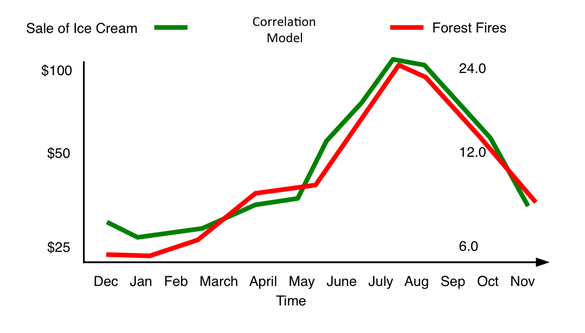
\includegraphics[width=0.6 \textwidth]{figures/corr_caus.png}
\caption{an example of correlation \href{https://www.decisionskills.com/blog/how-ice-cream-kills-understanding-cause-and-effect}{(source)}}
\end{figure}

Without having any information about what we are trying to model, we might conclude that there is a cause-effect relationship between these two measures. The graph also shows a correlation close to 1 for the two curves. When we start to analyse the data in details, the first thing that comes to our mind is that there is no logical relationship (and thus no cause-effect relationship) between the sale of ice cream and the forest fires. However, we can see clearly in the graph that the values are higher between May and November (with a peak in July) compared to the rest of the year. In fact, the heat is the reason behind forest fires and the sale of ice cream. We can then conclude the following : 

\begin{itemize}
\item[--] a causation between the heat and the sale of ice cream;
\item[--] a causation between the heat and the forest fire;
\item[--] a correlation between the sale of ice cream and the sale of ice cream.
\end{itemize}

This simple example shows us that, in general and without having a good knowledge about the problem, we tend to assume simple correlations between 2 variables when in fact there is a third variable that causes both of them. This is a core idea in causal inference : unlike for correlation, we can not rely only on the distribution of the data, even at the population level, but we also should rely on causal assumption that is always not testable in observational studies.\cite{pearl2010mathematics} 

	\subsubsection{Definitions}
	
The previous example shows a clear difference between causation and correlation. More generally, correlation is a special example of an association concept. The definition of these two concepts is given by Judea Pearl\cite{pearl2010mathematics, pearl2009causal} as follows :

\begin{itemize}
\item[--] An \textbf{associational concept} is any relationship that can be defined in terms of a joint distribution of observed variables. For example: regression, correlation.
\item[--] A \textbf{causal concept} is any relationship that cannot be defined from the distribution alone. One should also rely on causal assumption that explains the different relationships. For example: randomisation, confounding (it will be detailed later).
\end{itemize}


	\subsubsection{The difference between the 2 notions}

To have a better understanding of how causation and association differ, the following example is considered. The goal of a study is to test the effectiveness of a vaccine on a sick population. Let's denote by A the action of injecting the vaccine and by Y the effect of the vaccine on the population. In an association approach, the population will be divided into 2 groups : only one group will be injected with the vaccine. The effectiveness of the treatment is thus measured on the treated population ( $E[Y|A = 1]$ ) and it is also possible to see if the untreated population will be treated without the vaccine ( $E[Y|A = 0]$ ). However, in a causation approach, we suppose that is possible to inject the whole population and study the effect of the vaccine ( $E[Y^{a=1}]$ ) and at the same time, have the same population \textbf{not} injected ( $E[Y^{a=0}]$ ).

\begin{figure}[h]
\centering
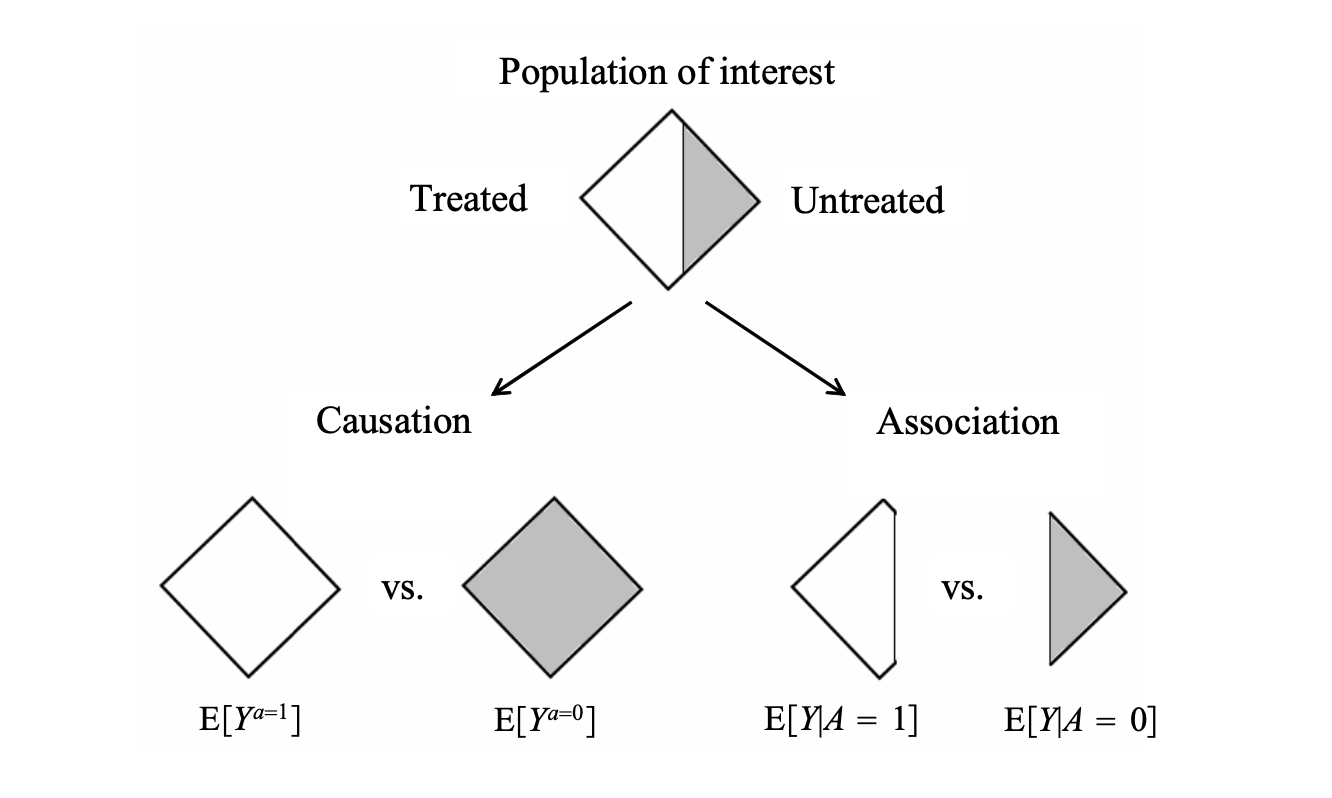
\includegraphics[width=0.6 \textwidth]{figures/asso_caus.png}
\caption{a visualisation of the difference between causation and association}
\end{figure}

One can see clearly the impossibility of applying in the causation approach : it is impossible to go back in time and inject an individual who was not injected; we can only observe one of the different potential outcomes. Meanwhile, there is some technics so that such an experiment can be possible: randomised experimentation is one example that will be detailed later.

%%%%%%%%%%%%%%%%%%%%%%%%%%%%%%%%%%

\subsection{Counterfactuals}

This is an important concept for causation. Counterfactuals could be defined as the answer to the question "what if ?" or simply as the unobserved outcome. If we consider the previous example in the case of an association, the unobserved outcomes will be the observations of "what if we have injected the proportion of the population that was not injected ?" and of "what if we have not injected the proportion of the population that was injected ?".

%%%%%%%%%%%%%%%%%%%%%%%%%%%%%%%%%%

\subsection{Confounders}

A confounding variable is an unmeasured variable that influences both the supposed cause and the supposed effect. Ignoring the confounder may lead to conclude an association between 2 variables when actually it is not the case. Confounders can also increase the variance or introduce biais.

Different technics exist to reduce the effect of the confounders (random samples, control variable ...)\footnote{An interesting article about confounders could be found at \href{https://www.statisticshowto.com/experimental-design/confounding-variable/}{www.statisticshowto.com}}. However, knowing in advance all the the confounders in the data/model is still very important.

\begin{figure}[h]
\centering
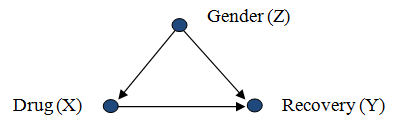
\includegraphics[width=0.5 \textwidth]{figures/confounding.png}
\caption{An example of a confounding variable : in this example, the Gender is not observed and it is affecting the variables Drug and Recovery}
\end{figure}

 %%%%%%%%%%%%%%%%%%%%%%%%%%%%%%%%%%
 
 \subsection{Simpson's paradox}

Simpson’s paradox, also called Yule-Simpson effect, in statistics, an effect that occurs when the marginal association between two categorical variables is qualitatively different from the partial association between the same two variables after controlling for one or more other variables.

\begin{figure}[h]
\centering
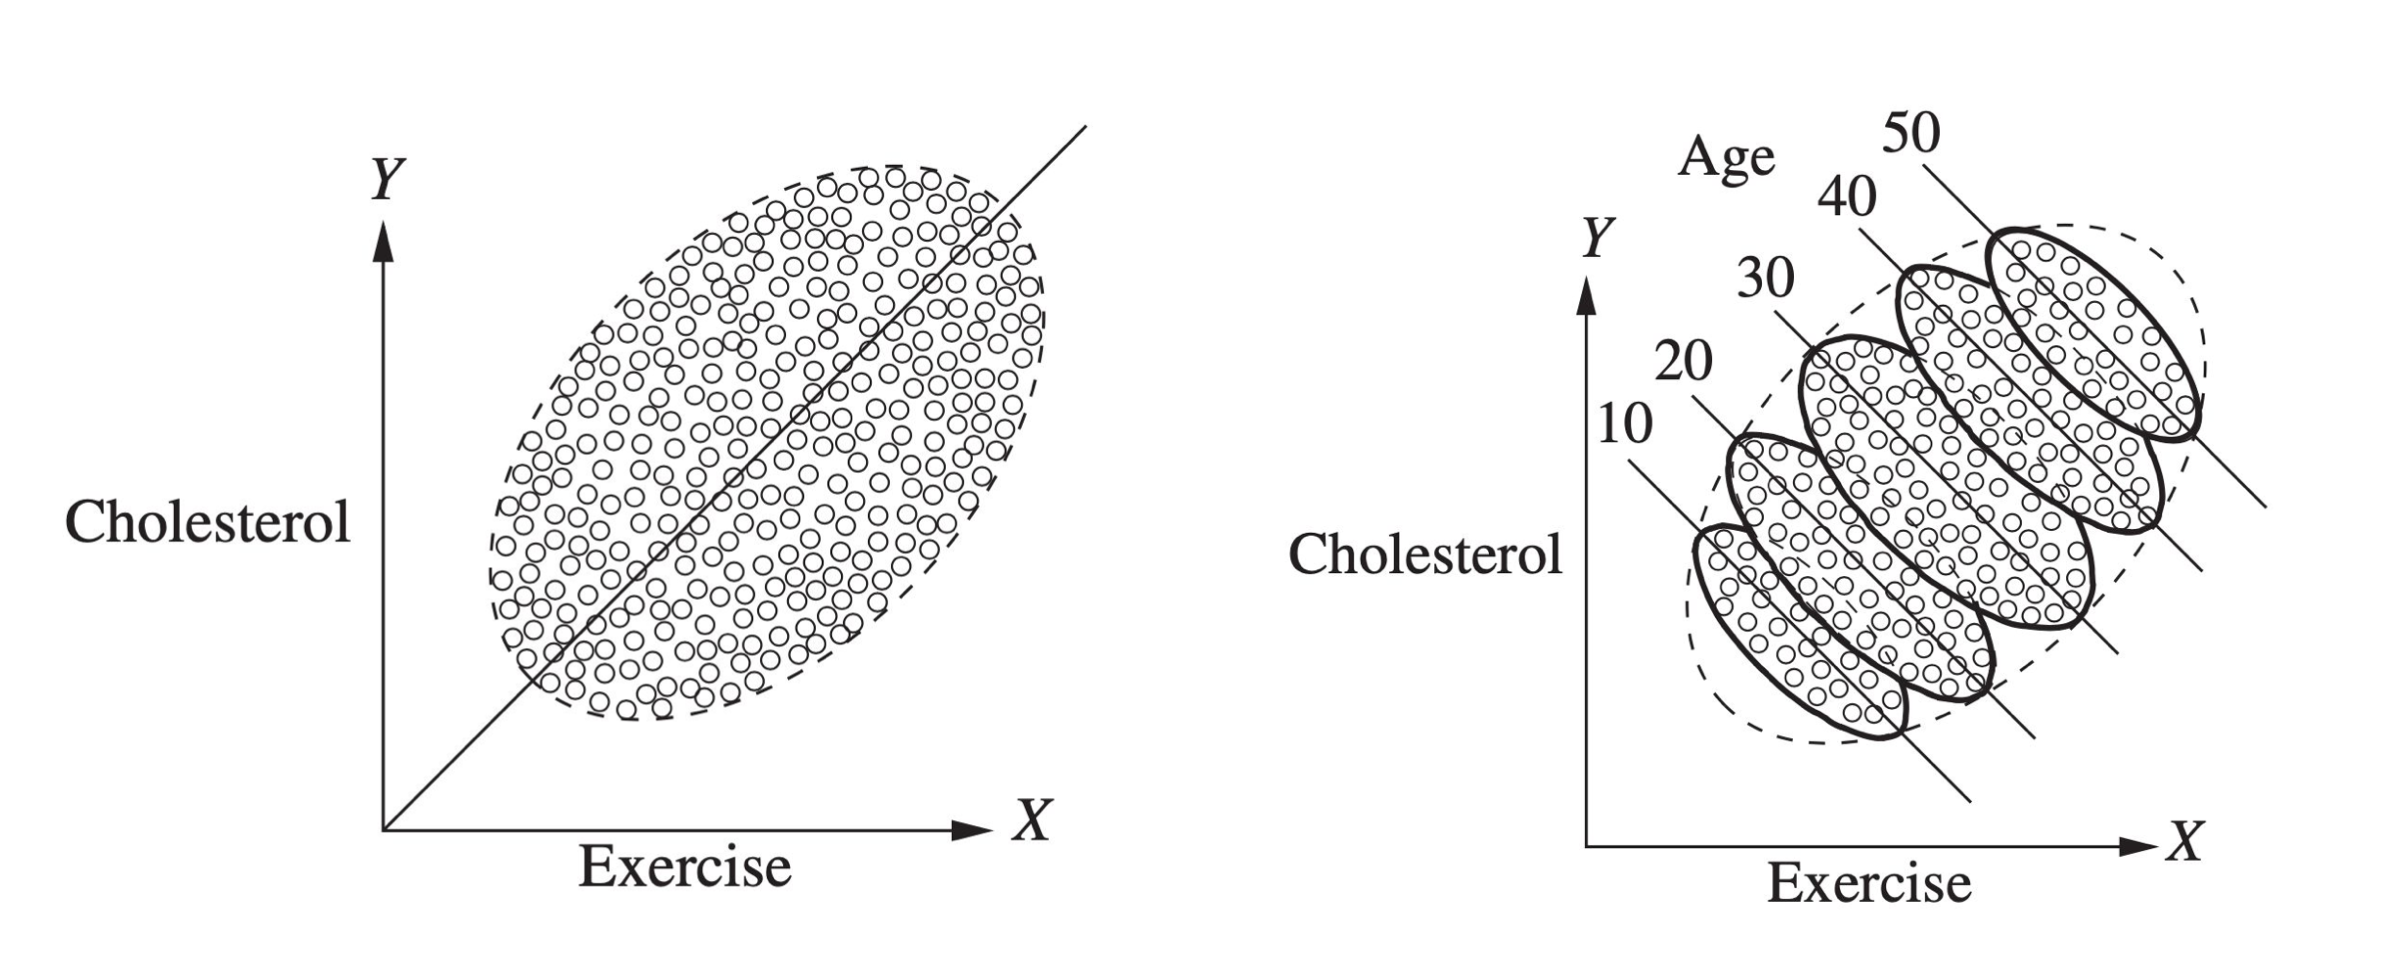
\includegraphics[width=0.7 \textwidth]{figures/simpson.png}
\caption{Illustration of the Simpson’s Paradox\cite{pearl2016causal}}
\end{figure}

The above example is one of the best illustration of the Simpson's paradox : when analysing the whole dataset, the first conclusion we can draw is that the amount of exercice is positively correlated with the level of cholesterol. Although, when including the information of age, we can see clearly, for every age category, a negative correlation between the two variables. Thus, domain knowledge is something very important when investigating the relationships in the data and sometimes the expected results are achieved only after increasing/decreasing the studied set of data - adding/excluding some variables.

\newpage 
%%%%%%%%%%%%%%%%%%%%%%%%%%%%%%%%%%

\section{Causal inference}

%%%%%%%%%%%%%%%%%%%%%%%%%%%%%%%%%%

\subsection{Average Causal Effect - ACE}

see \cite{hernan2020causal}


%%%%%%%%%%%%%%%%%%%%%%%%%%%%%%%%%%

\subsection{Individual level Causal Effect - ICE}

see \cite{hernan2020causal}

%%%%%%%%%%%%%%%%%%%%%%%%%%%%%%%%%%

\subsection{Fundamental Problem of Causal Inference}

- Missing data problem 


%%%%%%%%%%%%%%%%%%%%%%%%%%%%%%%%%%

\subsection{The Causal Hierarchy}


\begin{figure}[h]
\centering
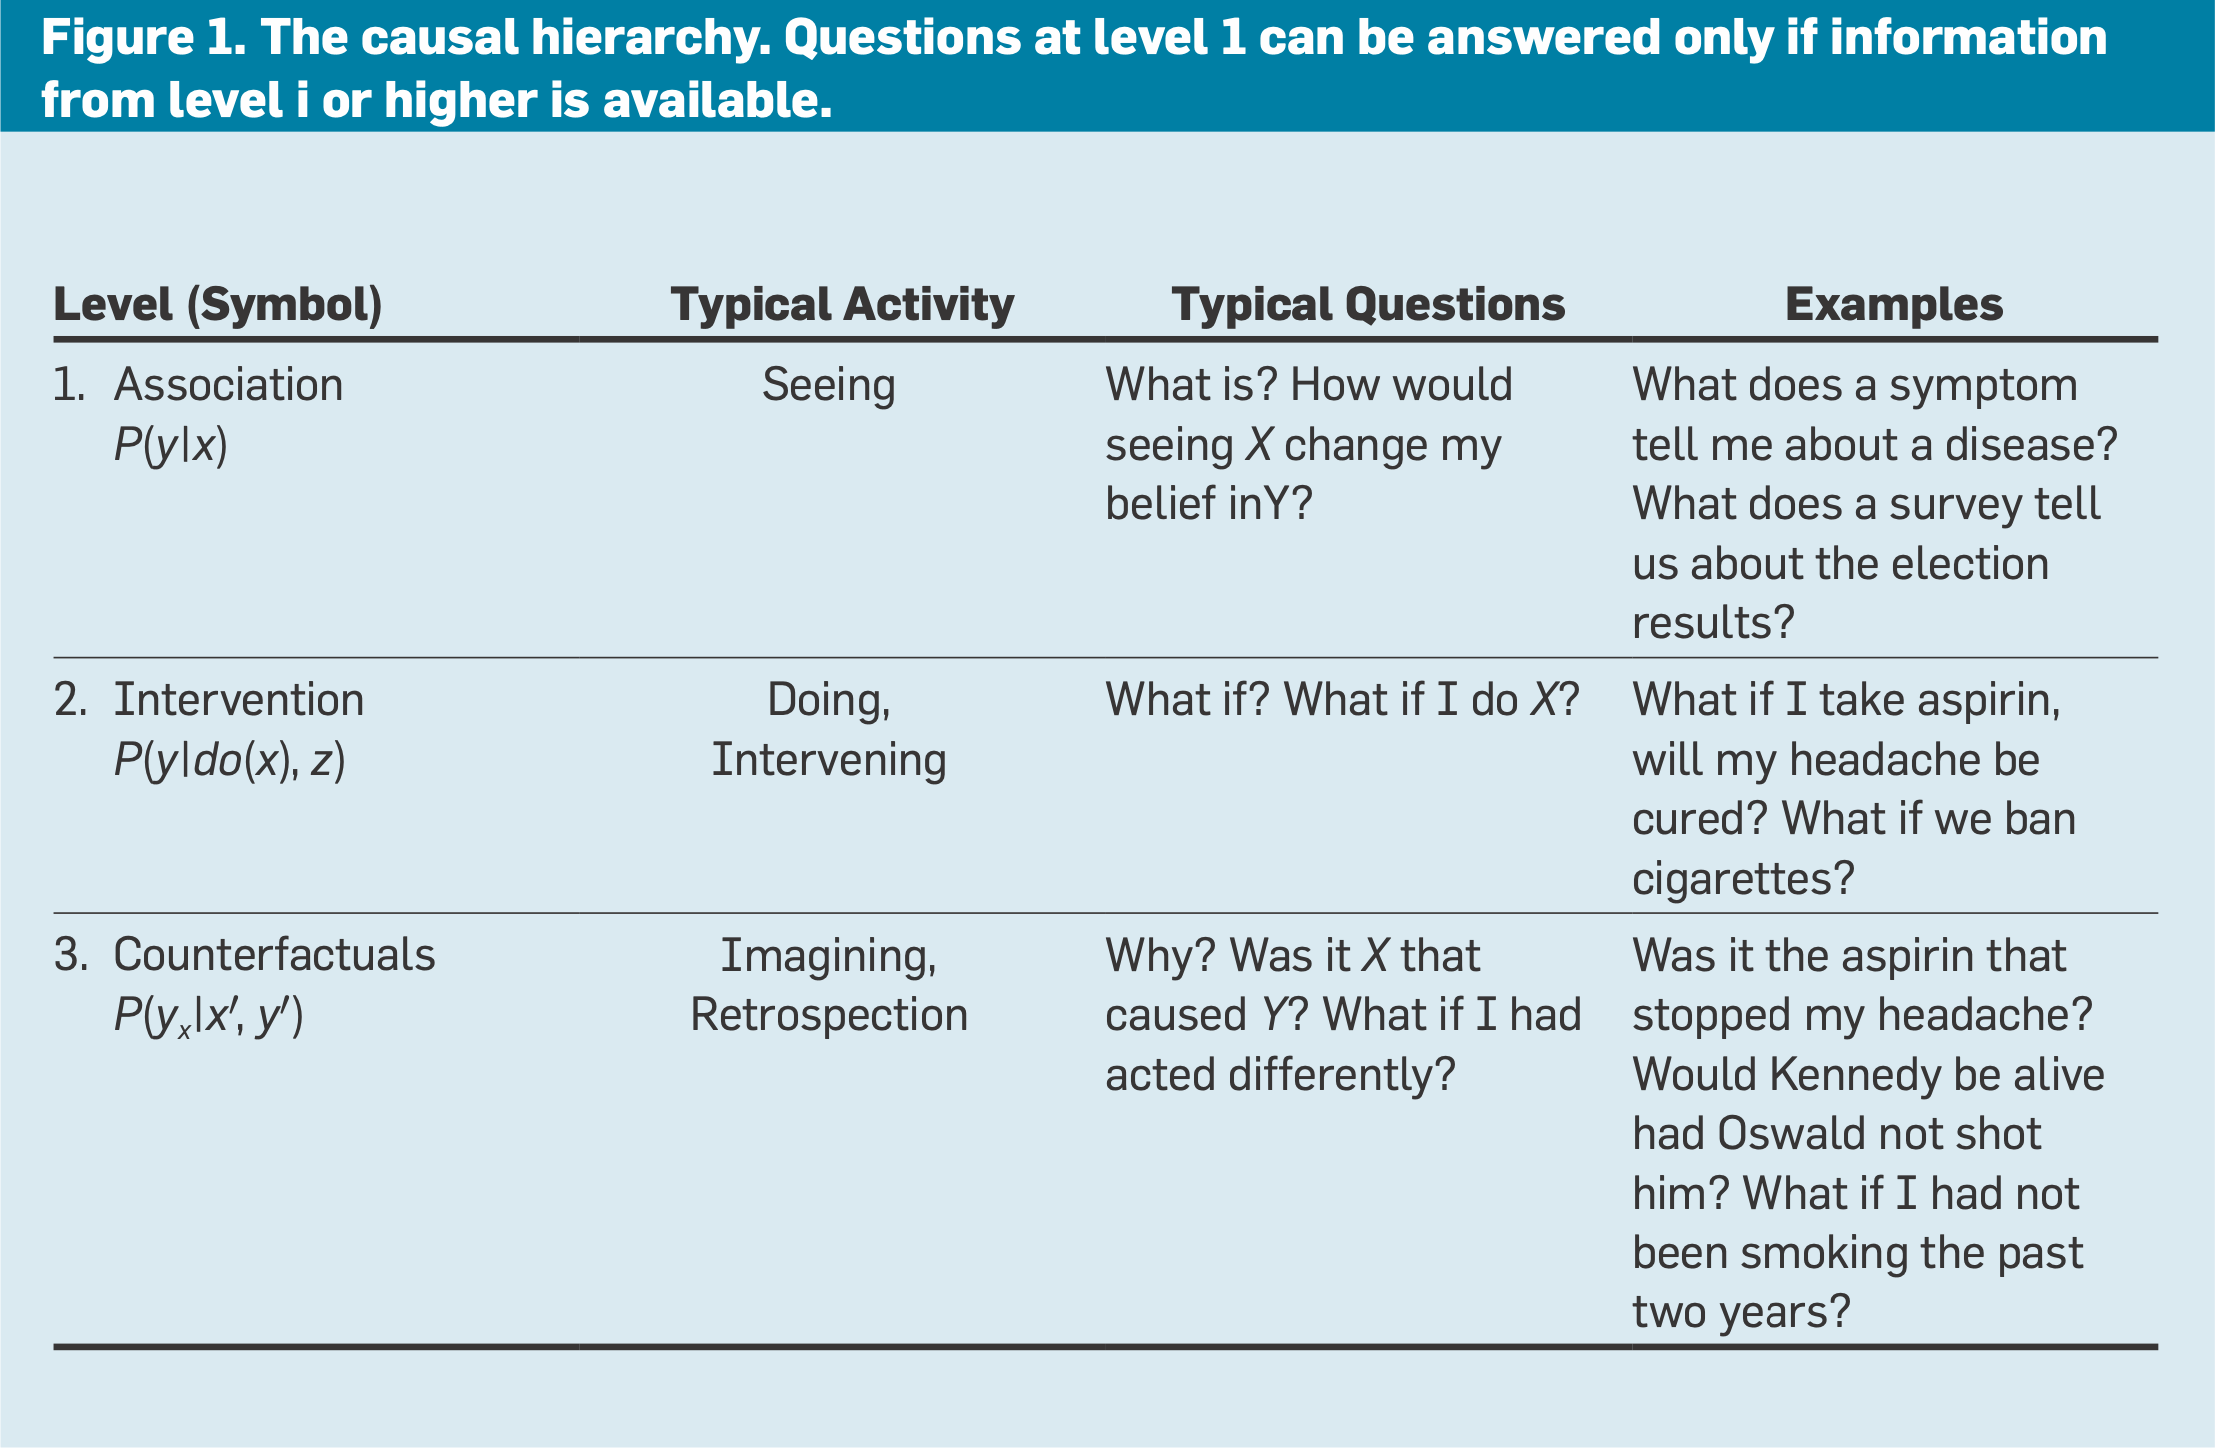
\includegraphics[width=0.7 \textwidth]{figures/asso_inter_caus.png}
\caption{The causal hierarchy\cite{pearl2019seven}}
\end{figure}


One of the very interesting papers that explains causal inference is : \href{https://cacm.acm.org/magazines/2019/3/234929-the-seven-tools-of-causal-inference-with-reflections-on-machine-learning/fulltext?mobile=false}{"The Seven Tools of Causal Inference, with Reflections on Machine Learning"} \cite{pearl2019seven}. This section is thus inspired mostly by this paper.

\cite{pearl2019seven} 
 
 
%%%%%%%%%%%%%%%%%%%%%%%%%%%%%%%%%% 
 \subsection{Graph representation}


\newpage 
%%%%%%%%%%%%%%%%%%%%%%%%%%%%%%%%%%

\section{Paper : Judea Pearl -- remove this}

see \cite{pearl2010mathematics} \\
One of the best paper so far. It explains clearly the difference between the causal concept and the associational concept (for example : correlation). The first concept ...


%% http://singapore.cs.ucla.edu/csl_papers.html     http://bayes.cs.ucla.edu/home.htm

%%%%%%%%%%%%%%%%%%%%%%%%%%%%%%%%%%

\section{Notations -- remove this}
see \cite{yao2020survey} and \cite{hernan2020causal}


%%%%%%%%%%%%%%%%%%%%%%%%%%%%%%%%%%

\section{Definition of the causality -- remove this}

Perhaps the most important message of the discussion and methods presented in this paper would be a widespread awareness that (1) all studies concerning causal relations must begin with causal assumptions of some sort and (2) that a friendly and formal language is currently available for articulating such assumptions.\cite{pearl2010mathematics}

\cite{rubin2005causal}


\newpage
%%%%%%%%%%%%%%%%%%%%%%%%%%%%%%%%%%

\section{Causal discovery}

A traditional way to discover causal relations is to use interventions or randomized experiments, which is, however, in many cases of interest too expensive, too time- consuming, unethical, or even impossible. Therefore, inferring the underlying causal structure from purely observational data, or from combinations of observational and experimental data, has drawn much attention in various disciplines. With the rapid accumulation of huge volumes of data, it is necessary to develop automatic causal search algorithms that scale well.\cite{10.3389/fgene.2019.00524}

%%%%%%%%%%%%%%%%%%%%%%%%%%%%%%%%%%

\section{Python Library : DoWhy}
library developed by Microsoft \cite{dowhy}, blog article available \href{https://www.microsoft.com/en-us/research/blog/dowhy-a-library-for-causal-inference/}{link}

%%%%%%%%%%%%%%%%%%%%%%%%%%%%%%%%%%

\newpage
\bibliographystyle{ieeetr} % plain : no order -- ieeetr : sorted
\nocite{*}    % print all references
\bibliography{reference/ref}

\end{document}
